\def\pgfsysdriver{pgfsys-dvisvgm.def}
% flashcards-title: Absolute and bounded evidence reports
% flashcards-desc: Report A claims universal proof. Report B states the studied organisms and conditions, a supported contribution, and one untested setting.
\documentclass[tikz,border=6pt]{standalone}
\usetikzlibrary{arrows.meta,calc,fit,positioning,shapes.geometric}

\definecolor{fcink}{HTML}{17212B}
\definecolor{fcblue}{HTML}{1D5D8C}
\definecolor{fcgreen}{HTML}{2D6A4F}
\definecolor{fcorange}{HTML}{A44A1F}
\definecolor{fcpale}{HTML}{F4F7F9}
\definecolor{fcsoil}{HTML}{8B5E3C}

\tikzset{
  fc text/.style={font=\sffamily, text=fcink},
  fc panel/.style={draw=fcink, line width=0.9pt, rounded corners=5pt, fill=fcpale},
  fc node/.style={draw=fcink, line width=0.9pt, rounded corners=4pt, fill=white,
    minimum width=24mm, minimum height=10mm, align=center, font=\sffamily},
  fc arrow/.style={-{Stealth[length=3.2mm,width=2.4mm]}, line width=1.2pt,
    draw=fcblue, line cap=butt},
  fc boundary/.style={draw=fcorange, line width=1.4pt, dash pattern=on 5pt off 3pt,
    rounded corners=7pt},
  fc label/.style={font=\sffamily\bfseries, text=fcink},
  fc note/.style={font=\sffamily\small, text=fcink, align=center}
}

\begin{document}
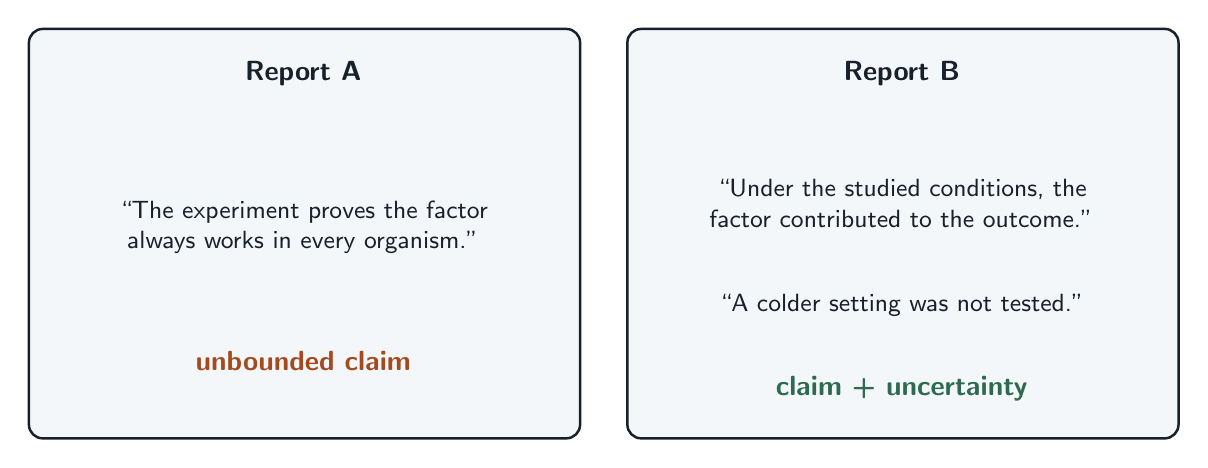
\begin{tikzpicture}[fc text, x=1cm, y=1cm]
  \node[fc panel, minimum width=70mm, minimum height=52mm, anchor=south west] at (0,0) {};
  \node[fc panel, minimum width=70mm, minimum height=52mm, anchor=south west] at (7.6,0) {};
  \node[fc label] at (3.5,4.65) {Report A};
  \node[fc note, text width=55mm] at (3.5,2.7) {``The experiment proves the factor always works in every organism.''};
  \node[fc label, text=fcorange] at (3.5,1.0) {unbounded claim};
  \node[fc label] at (11.1,4.65) {Report B};
  \node[fc note, text width=57mm] at (11.1,3.0) {``Under the studied conditions, the factor contributed to the outcome.''};
  \node[fc note, text width=57mm] at (11.1,1.7) {``A colder setting was not tested.''};
  \node[fc label, text=fcgreen] at (11.1,.65) {claim + uncertainty};
\end{tikzpicture}
\end{document}
